\documentclass[12pt]{report}

\usepackage{listings}
\usepackage{xcolor}
\usepackage{graphicx}
\usepackage{amsmath}
\usepackage{hyperref}
\usepackage{geometry}
\usepackage{subfig}
\usepackage{float}
\usepackage{pgfplots}

\geometry{a4paper, margin=1in}
\pgfplotsset{compat=1.18}

\definecolor{codegray}{gray}{0.95}
\definecolor{codegreen}{rgb}{0.0, 0.5, 0.0}
\definecolor{codepurple}{rgb}{0.5, 0, 0.4}

\lstdefinestyle{cppstyle}{
    language=C++,
    backgroundcolor=\color{codegray},
    basicstyle=\ttfamily\footnotesize,
    keywordstyle=\color{codepurple}\bfseries,
    stringstyle=\color{orange},
    commentstyle=\color{codegreen},
    numbers=none,
    tabsize=4,
    showspaces=false,
    showstringspaces=false,
    frame=single,
    framerule=0.8pt,
    framesep=5pt,
    aboveskip=0.5cm,
    belowskip=0.5cm,
}

\begin{document}

\title{\textbf{Bitonic Sort with CUDA}}
\author{\textbf{Savvas Tzanetis} \\ 10889}
\maketitle

\tableofcontents

\chapter{Abstract}
This report is part of an assignment for the \textbf{Parallel and Distributed Systems} class of the
Aristotle University's Electrical and Computer Engineering department. 

This project implements \textit{distributed sorting} using the \textbf{Bitonic Sort} algorithm with the use of the \textbf{CUDA} platform. The primary objective is to sort a dataset of $N = 2^q$ numbers (where $q \in N$). The implementation employs parallel processing to achieve efficient sorting, making it suitable for large-scale data sets.\\ \\
The code for this project is available at this \textcolor{blue}{\href{https://github.com/stzanetis/BitonicSortCUDA}{GitHub repository}} page.

\chapter{Serial Bitonic}
    To grasp the concept of distributed \textbf{Bitonic Sort}, it is essential to first understand its serial implementation. This foundational knowledge will provide the necessary context for comprehending the distributed version of the algorithm.

\section{Explanation}
    \textbf{Bitonic Sort} is a sorting algorithm that operates by sorting and merging bitonic sequences. A bitonic sequence is defined as a sequence of numbers that first monotonically increases and then monotonically decreases (or vise versa), or can be cyclically rotated to exhibit this pattern. Note that sorted sequences are also bitonic. For example, the sequence $6, 4, 3, 1, 2, 5, 8, 7$ is bitonic because it can be rotated to $7, 6, 4, 3, 1, 2, 5, 8$. 

    The algorithm is has the following characteristics:
    \begin{itemize}
        \item $log(n)$ steps, where n is the total amount of numbers, with $log(step)$ comparison phases in each step.
        \item In each comparison phase, we swap elements using the \textbf{min-max} criteria. The min-max pattern is presented in the image bellow:
    \end{itemize}

    \begin{figure}
        \centering
        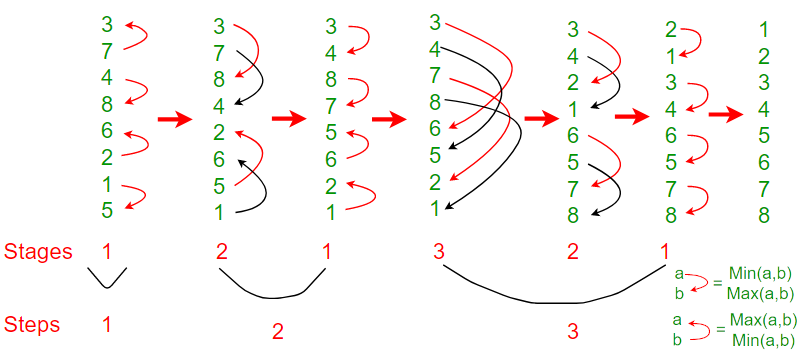
\includegraphics[width=0.9\linewidth]{bitonic.png}
        \caption{Bitonic Sort}
        \label{fig:enter-label}
    \end{figure}
    \section{Example}

    To illustrate the process, consider the following random sequence:
    \[S\{ 3,7,4,8,6,2,1,5 \}\]
    In each step each element is compared to its neighbor with distance \textbf{stage}.

    \begin{enumerate}
        \item \textbf{Step 1, Stage 1}
        \textbf{min-max pattern:} $min\:max\:max\:min\:min\:max\:max\:min$
        \[
            S\{3,7,8,4,2,6,5,1\}
        \] 
        \item \textbf{Step 2, Stage 2}
        \textbf{min-max pattern:} $min\:min\:max\:max\:max\:max\:min\:min$
        \[
            S\{3,4,8,7,5,6,2,1\}
        \]
        \item \textbf{Step 2, Stage 1}
        \textbf{min-max pattern:} $min\:max\:min\:max\:max\:min\:max\:min$
        \[
            S\{3,4,8,7,6,5,2,1\}
        \]
        \item \textbf{Step 3, Stage 3}
        \textbf{min-max pattern:} $min\:min\:min\:min\:max\:max\:max\:max$
        \[
            S\{3,4,2,1,6,5,7,8\}
        \]
        \item \textbf{Step 3, Stage 2}
        \textbf{min-max pattern:} $min\:min\:max\:max\:min\:min\:max\:max$
        \[
            S\{2,1,3,4,6,5,7,8\}
        \]
        \item \textbf{Step 3, Stage 1}
        \textbf{min-max pattern:} $min\:max\:min\:max\:min\:max\:min\:max$
        \[
            S\{1, 2, 3, 4, 5, 6, 7, 8\}
        \]
    \end{enumerate}

\section{Remarks}
    \begin{enumerate}
        \item The complexity of this algorithm is $O(nlog^2n)$. While it is higher than other popular sorting algorithms like \textbf{Merge Sort} or \textbf{Quick Sort},  \textbf{Bitonic Sort} is ideal for parallel implementation, because it always compares elements in a predefined sequence and the sequence of comparison does not depend on data. 
        \item \textbf{Bitonic Sort} can only be used if the number of elements to sort is $2^n$. The procedure fails if the number of elements is not in the aforementioned quantity precisely.
    \end{enumerate}
        
\chapter{Distributed Bitonic}
As mentioned above, this algorithm, when implemented in a serial manner, has a time complexity of \(\boldsymbol{O(n\log^2(n))}\), which is higher than most sorting algorithms. Despite that, this algorithm is useful, as it is well-suited for parallel implementations, like the one we will be discussing. For a parallel implementation, we can achieve a time complexity of \(\boldsymbol{O(\log^2(n))}\), which is significantly faster than our serial implementation. We will be achieving this goal by utilizing the \textbf{CUDA} platform for \textit{GPUs}.\\ \\
This assignment was split across three versions that needed to be implemented, each one being more advanced than the previous. More specifically:
\begin{itemize}
    \item \textbf{V0: }In this first version we were tasked with implementing a kernel where each thread only compares and exchanges. Being easy to write, but requiring too many function calls and global synchronizations.
    \item \textbf{V1: }The second version needed to be faster than V0. More specifically we needed to create an implementation that required fewer calls global synchronizations.
    \item \textbf{V2: }Lastly, we where tasked to modify the kernel of V1 to work with local memory instead of global for even faster results.
\end{itemize}

\section{Generating Random Sequences}
The sequences we used to test our results were generated using the \textbf{rand()} function, which is part of the \textbf{C++ standard library}. More specifically, we selected \textit{integers} ranging from \textbf{1} to \textbf{999} for simplicity.
\begin{lstlisting}[style=cppstyle]
void generateArray(int *values, int N) {
    std::srand(std::time(0));

    for (int i = 0; i < N; i++) {
        values[i] = std::rand() % 1000; // 0 - 999
    }
}
\end{lstlisting}

\section{Synchronization}
For a parallel implementation of the serial algorithm, we need to implement a method to exchange data between each sub-array for every step of the algorithm.

In \textbf{CUDA}, this is achieved by calling a function that will be executed by every thread inside a block, and synchronizing the results after each iteration.
\begin{lstlisting}[style=cppstyle]
for (int stage = 2; stage <= N; stage <<= 1) {
    for (int step = stage >> 1; step > 0; step = step >> 1) {
        bitonicSortStep<<<blocks, threads_per_block>>>
                (dev_values, stage, step);
        cudaDeviceSynchronize();
    }
}
\end{lstlisting}

\section{Exchanging Data Between Partners}
Data exchanges are done after each thread calculates its \textit{partner}. This is done using the logical operation \textbf{XOR} \textit{(tid \^ step)}. The threads are arranged in a \textit{hypercube-like} structure, where the global \textbf{ID} of each thread is treated as a binary number. The \textbf{XOR} operation between two binary numbers results in a number where the bits are set to $1$ at positions where the two numbers differ. The distance between two nodes in a hypercube is the number of differing bits between their binary representations, known as the \textbf{Hamming Distance}.
\begin{figure}[!h]
    \centering
    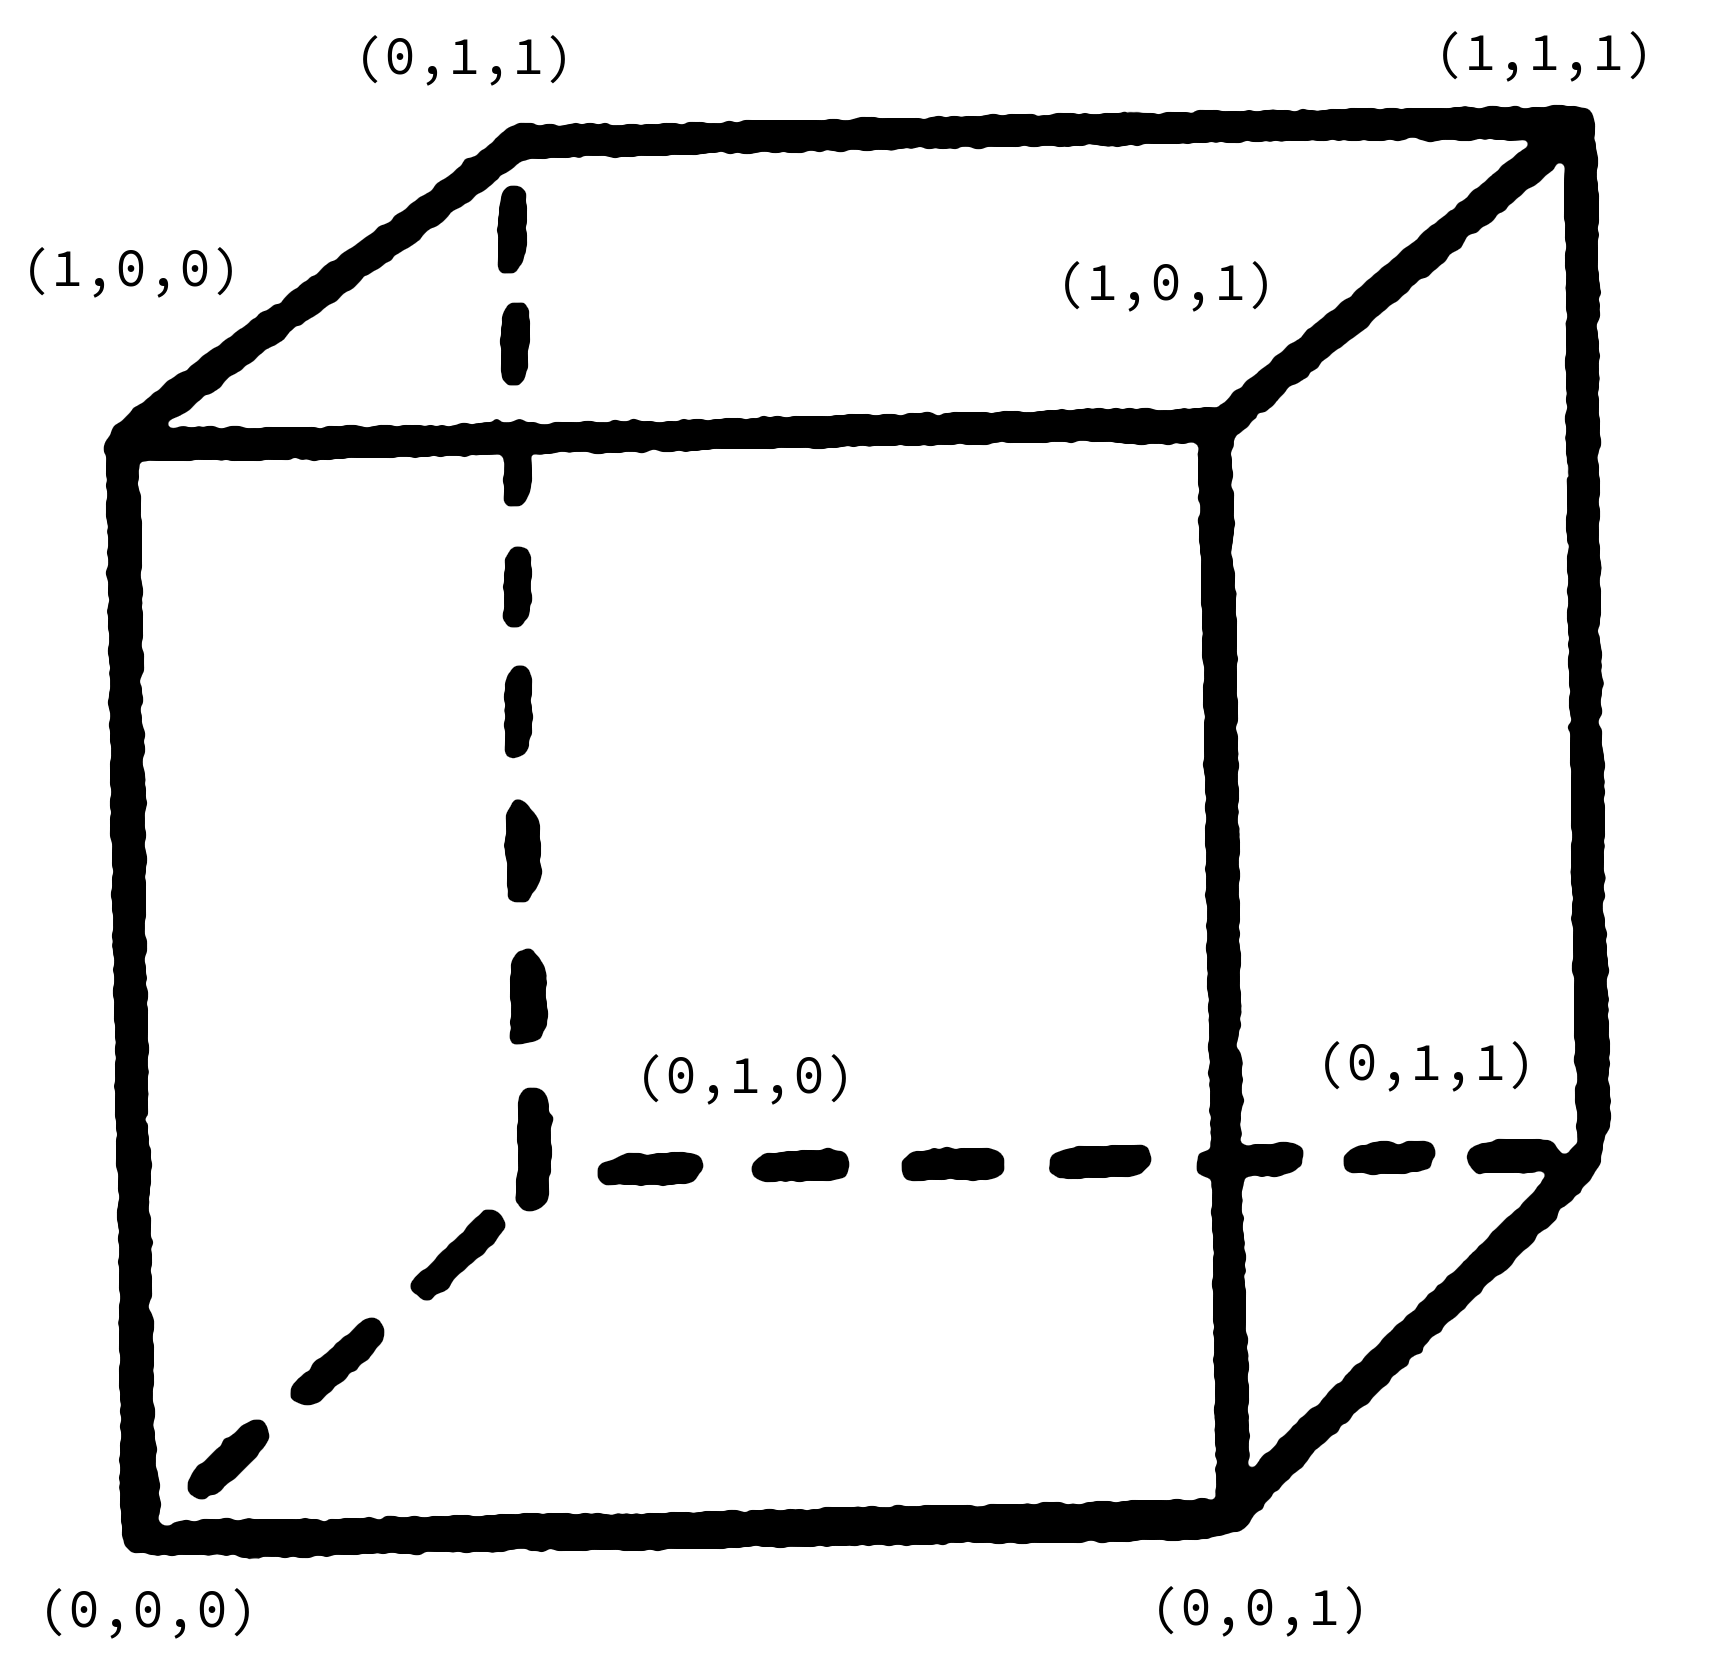
\includegraphics[width=0.5\linewidth]{cube.png}
    \caption{Enter Caption}
    \label{fig:enter-label}
\end{figure}

\newpage
\section{V0}
This first version of our parallel implementation is very simple. Using the simple concepts mentioned above, a significant improvement compared to a serial implementation is observed. But, while its performance is significantly faster, it still has downsides. Launching kernels multiple times can incur additional overhead, as each launch involves setting up the execution environment on the GPU. Also, multiple synchronizations need to be established, and considering that global synchronizations are generally slow operations, there is a big room for improvement in this implementation.

\section{V1}
The V1 version of the bitonic sort implementation introduces several key differences compared to the initial version. One of the most notable changes is the introduction of a second kernel, \textbf{localSort}, which is executed alongside the \textbf{bitonicSortStep} kernel we see in the first version (V0). The \textbf{localSort} function is designed to handle the initial sorting of elements within each block by using shared memory for faster data access and reducing the need for frequent global memory calls.

By performing local sorting within each block, the \textbf{localSort} kernel helps to set up the array for the subsequent stages of the bitonic sort.

\begin{lstlisting}[style=cppstyle]
void bitonicSort(int *values, int N) {
    int *dev_values;
    size_t size = N * sizeof(int);
    int threads_per_block = 1024;
    int blocks = ((N/2) - 1) / threads_per_block + 1;

    cudaMalloc((void**)&dev_values, size);
    cudaMemcpy(dev_values, values, size, cudaMemcpyHostToDevice);

    localSort<<<blocks, threads_per_block>>>
            (dev_values, N, 2, 1);

    for (int stage = 2048; stage <= N; stage <<= 1) {
        for (int step = stage >> 1; step > 512; step >>= 1) {
            bitonicSortStep<<<blocks, threads_per_block>>>
                    (dev_values, (N/2), stage, step);
            cudaDeviceSynchronize();
        }
        localSort<<<blocks, threads_per_block>>>
                (dev_values, N, stage, 512);
    }    

    cudaMemcpy(values, dev_values, size, cudaMemcpyDeviceToHost);
    cudaFree(dev_values);
}
\end{lstlisting}

\newpage
\section{V2}
The last version of our algorithm improves upon the \textit{V1} version by utilizing local memory instead of global. This is done inside the \textbf{localSort} kernel that we discussed about in the previous version by copying data into shared memory at the beginning, allowing threads within the same block to access data more quickly and efficiently. After the local sorting, the data is written back to global memory, minimizing the overhead associated with frequent global memory accesses.
\begin{lstlisting}[style=cppstyle]
__global__ void localSort(int *dev_values, int N, int stage, int step) {
    extern __shared__ int shared_values[];
    unsigned int tid = threadIdx.x + blockDim.x * blockIdx.x;
    unsigned int offset = N >> 1;
    unsigned int local_tid = threadIdx.x;

    shared_values[local_tid] = dev_values[tid];
    shared_values[local_tid + min(offset, blockDim.x)] = 
                                dev_values[tid + offset];
    __syncthreads();
}
\end{lstlisting}
\chapter{Results}
As previously mentioned, a serial version of this algorithm has a time complexity of $\boldsymbol{O(n \log^2(n)}$, which is not ideal, as there are faster algorithms. However, a parallel or distributed version, significantly lessens this to $\boldsymbol{O(\log^2(n))}$.

\begin{table}[h!]
    \centering
    \begin{tabular}{|c|c|c|c|}
        \hline
        \rule{0pt}{3ex}\textbf{Performance Table} & \textbf{Serial}                 & \textbf{Distributed}          & \textbf{Quick Sort}          \\ \hline
        \rule{0pt}{3ex}Time Complexity            & \(\boldsymbol{O(n \log^2(n))}\) & \(\boldsymbol{O(\log^2(n))}\) & \(\boldsymbol{O(n\log(n))}\) \\ \hline
    \end{tabular}
    \caption{Performance Table}
    \label{tab:simple_table}
\end{table}

\begin{center}
    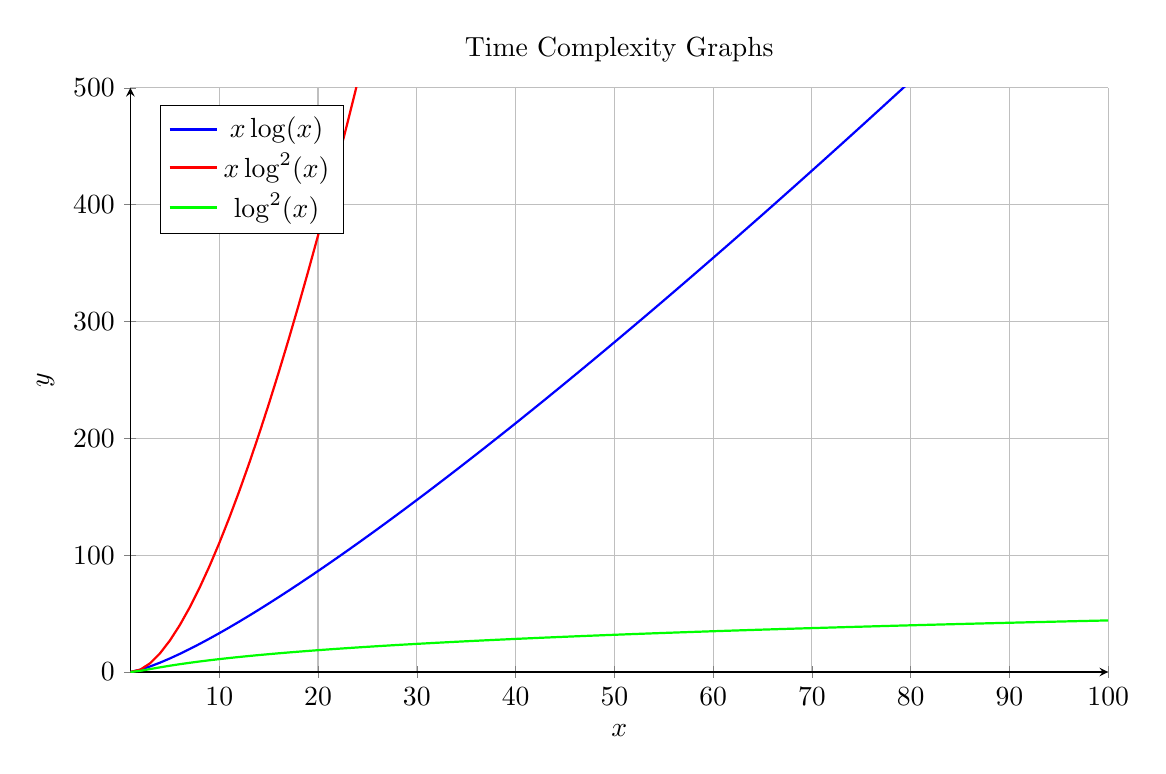
\begin{tikzpicture}
        \begin{axis}[
            width=14cm,
            height=9cm,
            xlabel={$x$},
            ylabel={$y$},
            xmin=1, xmax=100,
            ymin=0, ymax=500,
            legend pos=north west,
            grid=major,
            axis x line=bottom,
            axis y line=left,
            title={Time Complexity Graphs}
        ]
            % plot x*log2(x)
            \addplot[blue, thick] expression[domain=1:100, samples=100]{x * ln(x)/ln(2)};
            \addlegendentry{$x \log(x)$}

            % plot x*(log2(x))^2
            \addplot[red, thick] expression[domain=1:100, samples=100]{x * (ln(x)/ln(2))^2};
            \addlegendentry{$x \log^2(x)$}

            % plot (log2(x))^2
            \addplot[green, thick] expression[domain=1:100, samples=100]{(ln(x)/ln(2))^2};
            \addlegendentry{$\log^2(x)$}
        \end{axis}
    \end{tikzpicture}
\end{center}

This program was executed on a \textbf{Windows 11} machine with a \textbf{NVIDIA Geforce RTX 3060 12GB} graphics card. We tested our program across a range of \textit{n} values ([20:29]) where the random array (to be sorted) was populated with integers in the range \textbf{1–999}. We then verified the correctness of the results by iterating through the array and comparing each element with the next one.

In the graphic below, we can see the results of each version of our implementation compared to \textbf{qsort} for aforementioned $N$ values range. This graphic was created using the \textit{test.py} script that is also available at this projects \textcolor{blue}{\href{https://github.com/stzanetis/BitonicSortCUDA}{GitHub repository}} .

\begin{figure}[H]
    \centering
    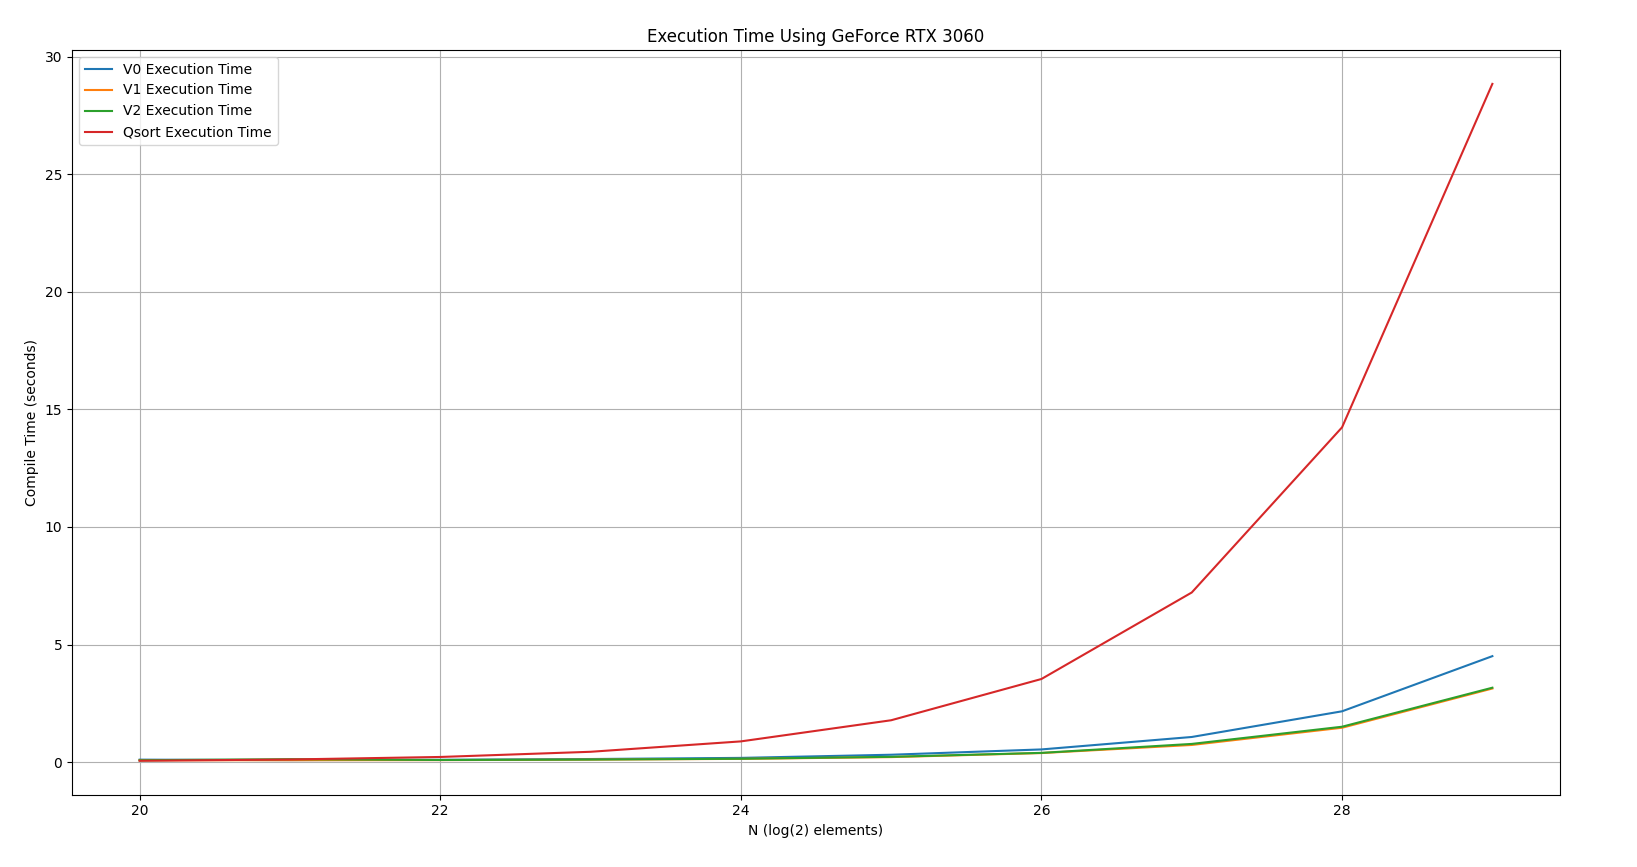
\includegraphics[width=1\linewidth]{results.png}
    \caption{Performance results}
    \label{fig:enter-label}
\end{figure}

\chapter{Tools and Sources}

In this project, the following tools where used:
\begin{enumerate}
    \item The \textbf{C++} programming language.
    \item The \textbf{CUDA} Library.
    \item \textbf{GitHub} for version control.
    \item \textbf{GitHub Copilot} as an AI assistant.
    \item \textbf{Python} with \textbf{matplotlib} for graphics
\end{enumerate}

The following sources were helpful for understanding the problem presented in the assignment:
\begin{itemize}
    \item \url{https://en.wikipedia.org/wiki/Bitonic_sorter}
    \item \url{https://www.geeksforgeeks.org/bitonic-sort/}
    \item Lecture notes from the \textbf{Parallel and Distributed Systems} course, written by professor \textbf{Nikolaos Pitsianis}.
\end{itemize}

\end{document}